%% Template for MLP Coursework 2 / 6 November 2017 

%% Based on  LaTeX template for ICML 2017 - example_paper.tex at 
%%  https://2017.icml.cc/Conferences/2017/StyleAuthorInstructions

\documentclass{article}
\usepackage[T1]{fontenc}
\usepackage{amssymb,amsmath}
\usepackage{txfonts}
\usepackage{microtype}

% For figures
\usepackage{graphicx}
\usepackage{subfigure} 

% For citations
\usepackage{natbib}

% For algorithms
\usepackage{algorithm}
\usepackage{algorithmic}

% the hyperref package is used to produce hyperlinks in the
% resulting PDF.  If this breaks your system, please commend out the
% following usepackage line and replace \usepackage{mlp2017} with
% \usepackage[nohyperref]{mlp2017} below.
\usepackage{hyperref}
\usepackage{url}
\urlstyle{same}

% Packages hyperref and algorithmic misbehave sometimes.  We can fix
% this with the following command.
\newcommand{\theHalgorithm}{\arabic{algorithm}}


% Set up MLP coursework style (based on ICML style)
\usepackage{mlp2019}
\mlptitlerunning{MLP Coursework 1 (\studentNumber)}
\bibliographystyle{icml2017}


\DeclareMathOperator{\softmax}{softmax}
\DeclareMathOperator{\sigmoid}{sigmoid}
\DeclareMathOperator{\sgn}{sgn}
\DeclareMathOperator{\relu}{relu}
\DeclareMathOperator{\lrelu}{lrelu}
\DeclareMathOperator{\elu}{elu}
\DeclareMathOperator{\selu}{selu}
\DeclareMathOperator{\maxout}{maxout}


%% You probably do not need to change anything above this comment

%% REPLACE this with your student number
\def\studentNumber{sXXXXXXX}

\begin{document} 

\twocolumn[
\mlptitle{MLP Coursework 1: Learning Algorithms and Regularization}

\centerline{\studentNumber}

\vskip 7mm
]

\begin{abstract} 
The abstract should be 100--200 words long,  providing a concise summary of the contents of your report.
\end{abstract} 

\section{Introduction}
\label{sec:intro}
This document provides a template for the MLP coursework 1 report.  This template structures the report into sections, which you are recommended to use, but can change if you wish.  If you want to use subsections within a section that is fine, but please do not use any deeper structuring.  In this template the text in each section will include an outline of what you should include in each section, along with some practical LaTeX examples (for example figures, tables, algorithms).  Your document should be no longer than \textbf{five pages},  with an additional page (or more!) allowed for references.

The introduction should place your work in context, giving the overall motivation for the work, and clearly outlining the research questions you have explored -- in this case questions arising from an investigation of learning rate algorithms, learning rate schedulers, and regularization/weight decay.  This section should also include a concise description of the Balanced EMNIST task and  data -- be precise: for example state the size of the training, validation, and test sets.

\section{Baseline systems} 
In this section you should report your baseline experiments for EMNIST.  No need for theoretical explanations of things covered in the course, but if you go beyond what was covered please explain what you did with references to relevant paper(s) if appropriate.   In this section you should aim to cover the both the ``what'' and the ``why'': \emph{what} you did, giving sufficient information (hyperparameter settings, etc.) so that someone else (e.g. another student on the course) could reproduce your results; and \emph{why} you performed the experiments you are reporting - what you are aiming to discover what is the motivation for the particular experiments you undertook. You should also provide some discussion and interpretation of your results.  

Your experimental sections should include graphs (for instance, figure~\ref{fig:sample-graph}) and/or tables (for instance, table~\ref{tab:sample-table})\footnote{These examples were taken from the ICML template paper.}, using the \verb+figure+ and \verb+table+ environments, in which you use \verb+\includegraphics+ to include an image (pdf, png, or jpg formats).  Please export graphs as 
\href{https://en.wikipedia.org/wiki/Vector_graphics}{vector graphics}
rather than \href{https://en.wikipedia.org/wiki/Raster_graphics}{raster
files} as this will make sure all detail in the plot is visible.
Matplotlib supports saving high quality figures in a wide range of
common image formats using the
\href{http://matplotlib.org/api/pyplot_api.html\#matplotlib.pyplot.savefig}{\texttt{savefig}}
function. \textbf{You should use \texttt{savefig} rather than copying
the screen-resolution raster images outputted in the notebook.} An
example of using \texttt{savefig} to save a figure as a PDF file (which
can be included as graphics in a \LaTeX document is given in the coursework document.

If you need a figure or table to stretch across two columns use the \verb+figure*+ or \verb+table*+ environment instead of the \verb+figure+ or \verb+table+ environment.  Use the \verb+subfigure+ environment if you want to include multiple graphics in a single figure.

\begin{figure}[tb]
\vskip 5mm
\begin{center}
\centerline{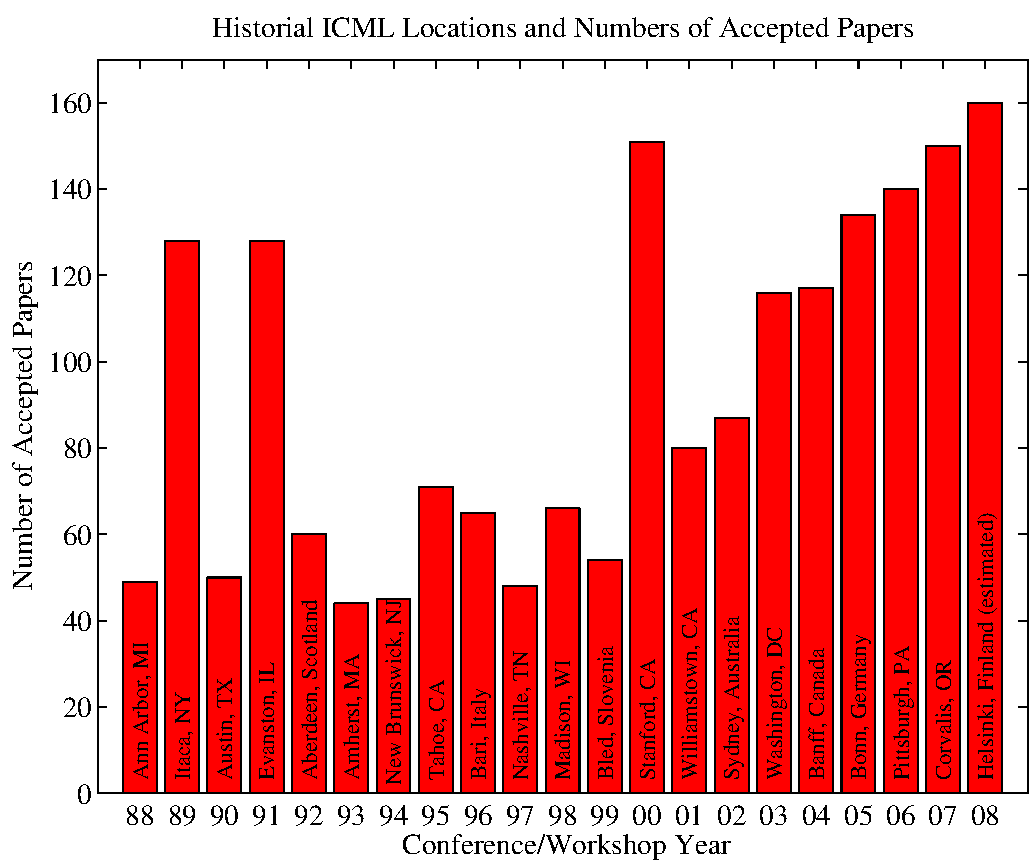
\includegraphics[width=\columnwidth]{icml_numpapers}}
\caption{Historical locations and number of accepted papers for International
  Machine Learning Conferences (ICML 1993 -- ICML 2008) and
  International Workshops on Machine Learning (ML 1988 -- ML
  1992). At the time this figure was produced, the number of
  accepted papers for ICML 2008 was unknown and instead estimated.}
\label{fig:sample-graph}
\end{center}
\vskip -5mm
\end{figure} 

\begin{table}[tb]
\vskip 3mm
\begin{center}
\begin{small}
\begin{sc}
\begin{tabular}{lcccr}
\hline
\abovespace\belowspace
Data set & Naive & Flexible & Better? \\
\hline
\abovespace
Breast    & 95.9$\pm$ 0.2& 96.7$\pm$ 0.2& $\surd$ \\
Cleveland & 83.3$\pm$ 0.6& 80.0$\pm$ 0.6& $\times$\\
Glass2    & 61.9$\pm$ 1.4& 83.8$\pm$ 0.7& $\surd$ \\
Credit    & 74.8$\pm$ 0.5& 78.3$\pm$ 0.6&         \\
Horse     & 73.3$\pm$ 0.9& 69.7$\pm$ 1.0& $\times$\\
Meta      & 67.1$\pm$ 0.6& 76.5$\pm$ 0.5& $\surd$ \\
Pima      & 75.1$\pm$ 0.6& 73.9$\pm$ 0.5&         \\
\belowspace
Vehicle   & 44.9$\pm$ 0.6& 61.5$\pm$ 0.4& $\surd$ \\
\hline
\end{tabular}
\end{sc}
\end{small}
\caption{Classification accuracies for naive Bayes and flexible 
Bayes on various data sets.}
\label{tab:sample-table}
\end{center}
\vskip -3mm
\end{table}





\section{Learning algorithms -- RMSProp and Adam}
In this section you should compare RMSProp and Adam with gradient descent, introducing these learning rules either as equations or as algorithmic pseudocode.  If you present the different approaches as algorithms, you can use the \verb+algorithm+ and \verb+algorithmic+ environments to format pseudocode (for instance, Algorithm~\ref{alg:example}). These require the corresponding style files, \verb+algorithm.sty+ and \verb+algorithmic.sty+ which are supplied with this package. 

\begin{algorithm}[ht]
\begin{algorithmic}
   \STATE {\bfseries Input:} data $x_i$, size $m$
   \REPEAT
   \STATE Initialize $noChange = true$.
   \FOR{$i=1$ {\bfseries to} $m-1$}
   \IF{$x_i > x_{i+1}$} 
   \STATE Swap $x_i$ and $x_{i+1}$
   \STATE $noChange = false$
   \ENDIF
   \ENDFOR
   \UNTIL{$noChange$ is $true$}
\end{algorithmic}
  \caption{Bubble Sort}
  \label{alg:example}
\end{algorithm}

You should, in your own words, explain what the different learning rules do, and how they differ.  You should then present your experiments and results, comparing and contrasting stochastic gradient descent, RMSProp, and Adam.  As before concentrate on the ``what'' (remember give enough information so someone can reproduce your experiments), the ``why'' (why did you choose the experiments that you performed -- you may have been motivated by your earlier results, by the literature, or by a specific research question), and the interpretation of your results.

In every section, you should present your results in a way that makes it easy for a reader to understand what they mean. You should facilitate comparisons either using graphs with multiple curves or (if appropriate, e.g. for accuracies) a results table. You need to avoid having too many figures, poorly labelled graphs, and graphs which should be comparable but which use different axis scales. A good presentation will enable the reader to compare trends in the same graph -- each graph should summarise the results relating to a particular research (sub)question.

Your discussion should interpret the results, both in terms of summarising the outcomes of a particular experiment, and attempting to relate to the underlying models. A good report would have some analysis, resulting in an understanding of why particular results are observed, perhaps with reference to the literature. Use bibtex to organise your references -- in this case the references are in the file \verb+example-refs.bib+.  Here is a an example reference \citep{langley00}.  

\section{Cosine annealing learning rate scheduler}
In this section you should present the cosine annealing scheduler,  supported using equations or algorithmic pseudocode.  Explain the approach in your own words.  Following this present your experiments, again remembering to include the ``what'', the ``why'', and the interpretation of results.  Again make sure you provide enough information about the hyperparameters to enable someone else to reproduce your results.

\section{Regularization and weight decay with Adam}
In this section you should present your experiments on regularization and weight decay with Adam.  In your own words explain the problem using L2 regularization with Adam (using both your own results and the discussion by \citet{loshchilov2018fixing}), and the solution proposed by \citeauthor{loshchilov2018fixing}.  Report the experiments you have carried out, being careful to be clear what research question is being addressed by each experiment -- again you should include \emph{what} experiments you performed (include details of hyperparameters, etc.),  \emph{why} you performed them (what was the motivation for the experiments, what research questions are you exploring), and the interpretation and discussion of your results.



\section{Conclusions}
\label{sec:concl}
Based on your experiments, what is the setup (models, algorithms) that produces your best system on the Balanced EMNIST data?  

You should draw conclusions from the experiments, related to the research questions outlined in the introduction (section~\ref{sec:intro}). You should state the conclusions clearly and concisely. It is good if the conclusion from one experiment influenced what you did in later experiments -- your aim is to learn from your experiments. Extra credit if you relate your findings to what has been reported in the literature.

A good conclusions section would also include a further work discussion, building on work done so far, and referencing the literature where appropriate.

\bibliography{example-refs}

\end{document} 

